\documentclass[
    ngerman,american
    ]{scrartcl}

    % ##########################################
    % special thanks to this template:  https://github.com/stefantruehl/research-proposal-template/blob/master/researchproposal.tex
    % # Choose the language for the document by editing below line
    % # de = German
    % # en = English
    \newcommand{\lang}{en}
    % ##########################################

    \usepackage{babel}
    \usepackage[utf8]{inputenc} 
    \usepackage{csquotes}
    \usepackage{enumitem}
    \usepackage{ifthen}
    \usepackage{lipsum}
    \usepackage{graphicx}
    \usepackage{hyperref}
    \usepackage[left=1in, right=1in, top=1in, bottom=1in]{geometry}

    \newcommand{\paperSubTitle}[1]
{
    \ifthenelse{\equal{#1}{en}}{Outline and Topic Proposal}{}
}

\newcommand{\sectionQuestions}[1]
{
    \ifthenelse{\equal{#1}{en}}{\section{Scope of Work and Study Area}}{}
}

\newcommand{\sectionQuestionsDescription}[1]
{
    \ifthenelse{\equal{#1}{en}}{In this section, I describe the proposed scope of work and the study area.}{}
}

\newcommand{\sectionInitialTOC}[1]
{
    \ifthenelse{\equal{#1}{en}}{\section{Relevant Datasets}}{}
}

\newcommand{\sectionInitialTOCDescription}[1]
{
    \ifthenelse{\equal{#1}{en}}{In this section, I outline the probable content of the final paper in probable sections.}{}
}

\newcommand{\sectionSource}[1]
{
    \ifthenelse{\equal{#1}{en}}{\section{Relevant Related Work}}{}
}


\newcommand{\sectionSourceDescription}[1]
{
    \ifthenelse{\equal{#1}{en}}{In this section, we'll talk about relevant related work.}{}
}

\newcommand{\questionOne}[1]
{
    \ifthenelse{\equal{#1}{en}}{What is the problem I want to address in this work?}{}
}

\newcommand{\questionTwo}[1]
{
    \ifthenelse{\equal{#1}{en}}{Why is it a problem?}{}
}

\newcommand{\questionThree}[1]
{
    \ifthenelse{\equal{#1}{en}}{What is my proposed solution?}{}
}

\newcommand{\questionFour}[1]
{
    \ifthenelse{\equal{#1}{en}}{Why is it a solution?}{}
}

    \ifthenelse{\equal{en}{\lang}}
    {
        \selectlanguage{american} 
    }{
        \ifthenelse{\equal{de}{\lang}}
        {
            \selectlanguage{ngerman}
        }
        {\selectlanguage{american}}        
    }

    \usepackage[round]{natbib}
    \renewcommand{\cite}[1]{ (\citeauthor{#1}, \citeyear{#1})}

    
    
    \usepackage{amsmath}
    \title{
        % ##########################################
        % # Insert the title of your paper/thesis here
        % ###### 
        % Coming up with a good title is hard.
        % It should:
        %  1. capture the contents of the your work
        %  2. not be to broad or generic
        %  3. stick to the truth and don't not oversell
        %  4. use established terms and wordings
        %  5. make people curious about your work
        %  6. use current buzzwords if possilbe (but do it right)
        %  7. not use too many buzzwords :-)
        Floatplane Accesible Lakes - A Survey with Google Earth Engine
        % ##########################################
        \\  \Large{\paperSubTitle{\lang}}} % don't touch this line

    \author{
        % ##########################################
        % # Your name goes here
        % ######
        % wWll, that should be obvious, right? 
        Patrick, Kai, Youji, Daniyah
        % ##########################################
        }
    
    \begin{document}
      \maketitle

        \section{Introduction}
        
            As part of this research project, I intend to use Google Earth Engine to identify potentially float plane accessible lakes throughout Alaska.  I intend to restrict the study area to the regions described in "Flight Plan for the Future" \cite{schwoerer2022flight}, but may further restrict the study area if the techniques for estimating accessible lakes become impractical or we become pressed for time.  For now, the region of interest should roughly match the mapped area in "Flight plan for the Future" \cite{schwoerer2022flight} visible in figure \ref{fig:tobymap}.  The polygon for the appropriate region at the current time of writing is is visible in figure \ref{fig:akpoly}.  At very minimum I think it would be good to investigate the amount of potentially floatplane accessible lakes in the Susitna Valley (see figure \ref{fig:susitna}) and slightly farther out along the Iditarod trail.



            \begin{figure}
                \centering
                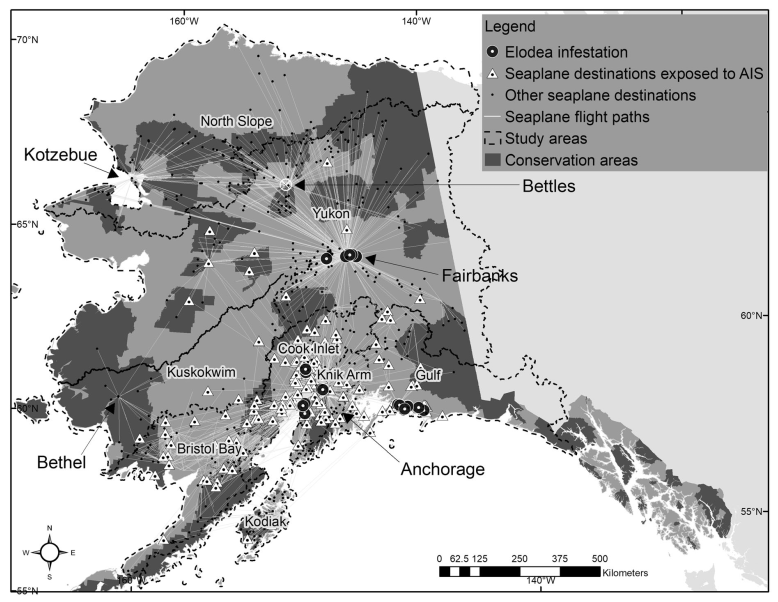
\includegraphics[width=0.75\linewidth]{tobymap.png}
                \caption{Map from "Flight plan for the future"}
                \label{fig:tobymap}
            \end{figure}



            \begin{figure}
                \centering
                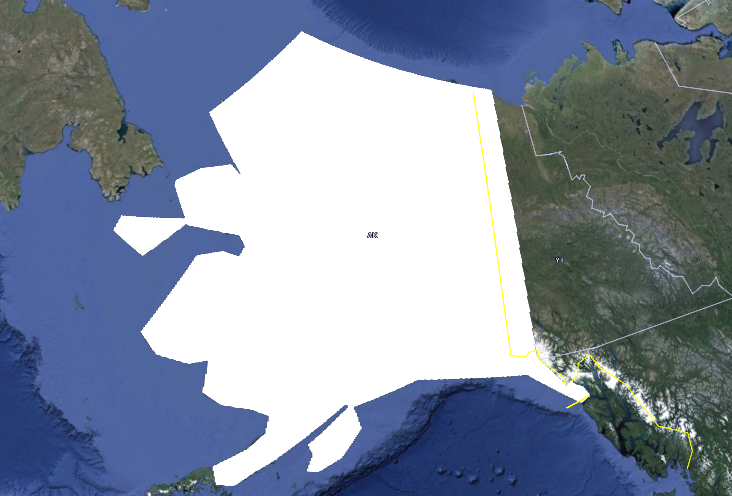
\includegraphics[width=0.75\linewidth]{polyimage.png}
                \caption{Proposed Polygon Visualized in Google Earth}
                \label{fig:akpoly}
            \end{figure}

            \begin{figure}
                \centering
                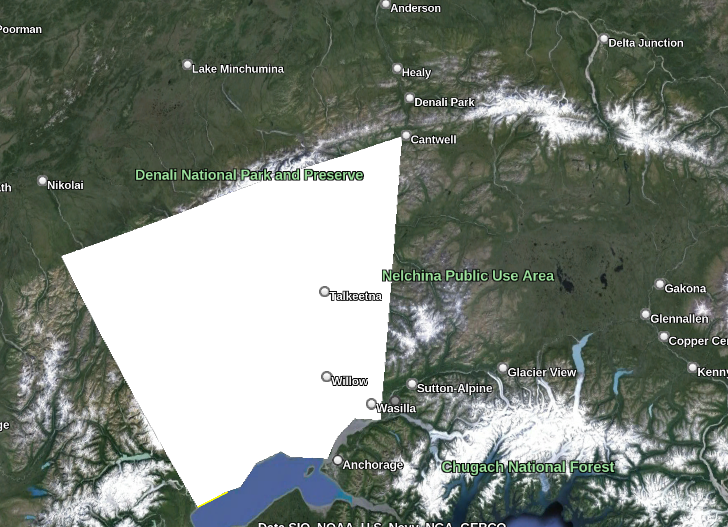
\includegraphics[width=0.75\linewidth]{susitnaroi.png}
                \caption{Backup Polygon if The Initial ROI is too Large}
                \label{fig:susitna}
            \end{figure}
            

        
        
            During my research for my thesis, I have not been able to find very many papers or articles about which lakes are potentially "floatplane" accessible.  There is a fantastic report from the BLM \cite{trammel2016} that has tried to quantify this variable for the Central Yukon Region, and another excellent paper where a survey of floatplane pilots was conducted \cite{schwoerer2022flight} which identified 682 known floatplane destinations, and there are numerous papers about detecting new lakes \cite{zhang2014lakes}, or monitoring lake area or even volume by satellite \cite{sima2013using}.  However, I have not seen much information about simply counting lakes by shape.

            Given that my research is directly concerned with the transmission of an invasive species on aircraft floats, having a mapping of waterbodies that are "floatplane accessible" would be helpful for future monitoring and mitigation strategies.  Simply being able to rule out certain waterbodies for survey could have major practical benefits.  If you cannot get there by boat, or floatplane, then monitoring the lake for infestations probably isn't necessary. There are multiple other potential benefits to attempting to count the number of lakes that can be reached by float equipped aircraft as well.

            Float equipped fixed-wing aircraft add a lot of economic value to the state of Alaska.  The one study I found about floatplane based tourism in Alaska was from 2007, but it estimated approximately a quarter million dollars in revenue per season just to Chichagof Island from Juneau \cite{dugan2007nature} excluding lodge flights.  Identifying potentially "unexplored" lakes could be financially beneficial to local air carriers developing packages to explore remote parts of Alaska.
            
            Similarly, because float equipped airplanes are typically significantly cheaper to operate than helicopters with similar payloads identifying locations close to resource extraction projects could provide significant cost savings or even reduce the environmental impact of building a runway for exploratory projects.  If this can be done for Alaska, it can be done in other locations worldwide.

            The ability to measure the geometry of lakes or other waterbodies has a lot of practical application in other types of research.  While I do not claim to be a hydrologist, the shape and contours of lakes and rivers are key to analyzing topics in natural resource management, environmental studies, and computational geometry.  If we can narrow down the count of lakes by their shape and geometry, that will be applicable to many other tasks where the shape of the object that is sensed remotely is important.

            Finally, given the notable lack of papers on this topic specifically (really only one or two), I believe this is an opportunity to conduct truly novel research on a topic that is simultaneously approachable and interesting.  Beyond the economic and cross-disciplinary reasons, floatplanes are "cool" aviation is "fun" and exploring remote parts of Alaska is enjoyable.  This study will allow us to conduct truly novel research while exploring an interesting topic.

        \section{Data}

        \section{Methodology}

        \section{Results}

        \section{Discussion}

        \section{Concluding Remarks}
                
        
        \section{References}

        
            \bibliographystyle{plainnat}
            \bibliography{bibliography}

\end{document}